\documentclass[pre,aps,superscriptaddress,nofootinbib]{revtex4}

\usepackage{amsmath,amsfonts,amssymb,bm,graphicx,hyperref,listings,xcolor,float,mathrsfs}
\usepackage{fontawesome5}
\setlength{\parindent}{0pt}

\begin{document}

\title{Polarisation-biased trajectories of independent Brownian rotors\\{\small Analytic considerations with Mathieu functions}}

\author{Yann-Edwin Keta}
\maketitle

\section{Scaled cumulant generating function and rate function}

We wish to bias the trajectories of the system with respect to the mean vectorial polarisation over a trajectory,
\begin{equation}
\bm{p}_{\tau} = \frac{1}{\tau} \int_0^{\tau} \text{d}t \, \bm{p}(t) = \frac{1}{N \tau} \int_0^{\tau} \text{d}t \, \sum_i \bm{u}(\theta_i(t)),
\end{equation}
and therefore need to compute the scaled cumulant generating function (SCGF)
\begin{equation}
N \psi_{\bm{p}}(\bm{s}) = \lim_{\tau \rightarrow \infty} \frac{1}{\tau} \log\left<\exp\left(- \bm{s} \cdot N \int_0^{\tau} \text{d}t \, \bm{p}(t)\right)\right>_0
\end{equation}
where we will assume that $\bm{s}$ is along the $x$-axis, and compute
\begin{equation}
\psi_ {p}(s) = \lim_{\tau \rightarrow \infty} \frac{1}{\tau} \log\left<\exp\left(- s N \int_0^{\tau} \text{d}t \, p_x(t)\right)\right>_0,
\end{equation}
from which we can recover
\begin{equation}
\psi_{\bm{p}}(\bm{s}) = \psi_{p}\left(\sqrt{s_x^2 + s_y^2}\right)
\end{equation}
from the fact that $\psi_{\bm{p}}(\bm{s})$ has to be cylindrically symmetric. We then have that $N \psi_s(p)$ is the largest eigenvalue of the eigenproblem
\begin{equation}
N \psi_{p}(s) P[\{\theta_i\}] = \mathscr{W}_{s, p} P[\{\theta_i\}],
\end{equation}
where we introduced the tilted generator \cite{touchette2018introduction}
\begin{equation}
\mathscr{W}_{s, p} = \mathcal{L} - s N p = D_r \sum_i \frac{\partial^2}{\partial \theta_i^2} - s \sum_i \cos\theta_i,
\end{equation}
using here $s \equiv s_x$ and $p \equiv p_x$, so that
\begin{equation}
\sum_i \left(\prod_{j \neq i} P(\theta_j)\right) \left[\psi_{p}(s) P(\theta_i) - \left(D_r \frac{\partial^2}{\partial \theta_i^2} P(\theta_i) - s \cos(\theta_i) P(\theta_i)\right)\right] = 0,
\end{equation}
is equivalent to the $1$-particle eigenproblem,
\begin{equation}
\psi_{p}(s) P(\theta) - \left(D_r \frac{\partial^2}{\partial \theta^2} P(\theta) - s \cos\theta P(\theta)\right) = 0 \Leftrightarrow \frac{\partial^2}{\partial \theta^2} \tilde{P}(\theta^{\prime}) + (a - 2 q \cos 2 \theta^{\prime}) \tilde{P}(\theta^{\prime}) = 0,
\label{1P_eigenproblem}
\end{equation}
with $2 \theta^{\prime} = \theta$, $\tilde{P}(\theta/2) = P(\theta)$, and
\begin{equation}
a = - \frac{4 \psi_{p}(s)}{D_r},~ q = \frac{2 s}{D_r},
\end{equation}
and which solutions are known as the Mathieu functions \cite{mathieu}.\\

Most notably, we have that for any $q \in \mathbb{R}$ there is a countable infinity of $a$. Inspired by \cite{grandpre2018current} we will choose $a_{\mathrm{Mathieu}, 0}(q)$ the characteristic value of the $0$-th Mathieu function which is $\pi$-periodic and even. We thus have the SCGF
\begin{equation}
N \psi_{\bm{p}}(\bm{s}) = N \psi_{p}\left(\sqrt{s_x^2 + s_y^2}\right) = - N \frac{D_r}{4} a_{\mathrm{Mathieu}, 0}\left(\frac{2}{D_r} \sqrt{s_x^2 + s_y^2}\right),
\end{equation}
and by Legendre transform
\begin{equation}
\begin{aligned}
N I(\bm{p}) &= \sup_{\bm{s} \in \mathbb{R}^2} \{- \bm{s} \cdot N \bm{p} - N \psi_{\bm{p}}(s)\}\\
&= \sup_{\bm{s} \in \mathbb{R}^2} \left\{- \bm{s} \cdot N \bm{p} + N \frac{D_r}{4} a_{\mathrm{Mathieu}, 0}\left(\frac{2}{D_r} \sqrt{s_x^2 + s_y^2}\right)\right\},
\end{aligned}
\end{equation}
we obtain the rate function. We note that both $\psi_{\bm{p}}(\bm{s})$ and $I(\bm{p})$ are cylindrically symmetric.\\

We have the following expansion of the SCGF for small $s$ \cite{abramowitz1948handbook},
\begin{equation}
\begin{aligned}
\psi_{\bm{p}}(\bm{s}) &= - \frac{D_r}{4} \left(-\frac{1}{2} \left(\frac{2}{D_r} \sqrt{s_x^2 + s_y^2}\right)^2 + \mathcal{O}(|\bm{s}|^4)\right),~ s \to 0\\
&= \frac{1}{2} (s_x^2 + s_y^2) \frac{1}{D_r} + \mathcal{O}(|\bm{s}|^4) ,~ s \to 0,
\end{aligned}
\end{equation}
and thus with
\begin{equation}
\begin{aligned}
\left(\frac{\partial^2}{\partial s_x^2} + \frac{\partial^2}{\partial s_y^2}\right) \psi_{\bm{p}}(\bm{s}) &= N \tau \left(\left<p_{x,\tau}^2 + p_{y,\tau}^2\right>_{\bm{s}} - \left<p_{x,\tau}\right>^2_{\bm{s}} - \left<p_{y,\tau}\right>^2_{\bm{s}}\right) = N \tau \left(\left<\bm{p}_{\tau}^2\right>_{\bm{s}} - \left<\bm{p}_{\tau}\right>^2_{\bm{s}}\right)\\
&= N \tau \mathrm{Var}(\bm{p}_{\tau})_{\bm{s}},
\end{aligned}
\end{equation}
we get
\begin{equation}
\mathrm{Var}(\bm{p}_{\tau})_0 = \frac{2}{N \tau D_r},
\end{equation}
and thus
\begin{equation}
\begin{aligned}
I(\bm{p}) &= \frac{1}{2} \bm{p} \cdot \begin{pmatrix} \left. \frac{\partial^2 I}{\partial p_x^2} \right|_0 & \left. \frac{\partial^2 I}{\partial p_x \partial p_y}  \right|_0 \\ \left. \frac{\partial^2 I}{\partial p_x \partial p_y}  \right|_0 & \left. \frac{\partial^2 I}{\partial p_y^2} \right|_0 \end{pmatrix} \bm{p} + \mathcal{O}(\bm{p}^4)\\
&= \frac{1}{2} D_r \bm{p}^2 + \mathcal{O}(\bm{p}^4),
\end{aligned}
\end{equation}
the rate function (see Fig. \ref{mathieu_rate_fig} \textbf{(left)}), considering $I(0) = 0$ and $I(\bm{p}) = I(-\bm{p})$.\\

We can compare the rate function to numerical results from the cloning simulations of Brownian rotors biased with respect to their squared polarisation, and the semi-analytical upper bound $-\inf_s \tilde{B}_{s,p^2}$ obtained in this case \cite{brownian_rotors_ldp} (see Fig. \ref{mathieu_rate_fig} \textbf{(right)}).

\begin{figure}[H]
\centering
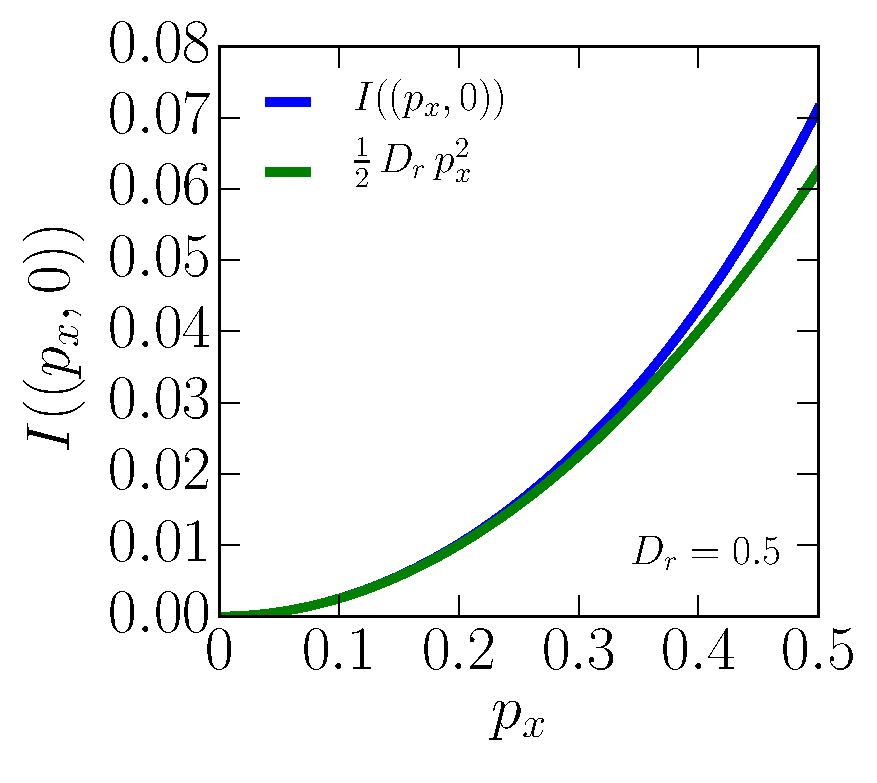
\includegraphics[width=0.40\textwidth]{mathieu_rate.eps}
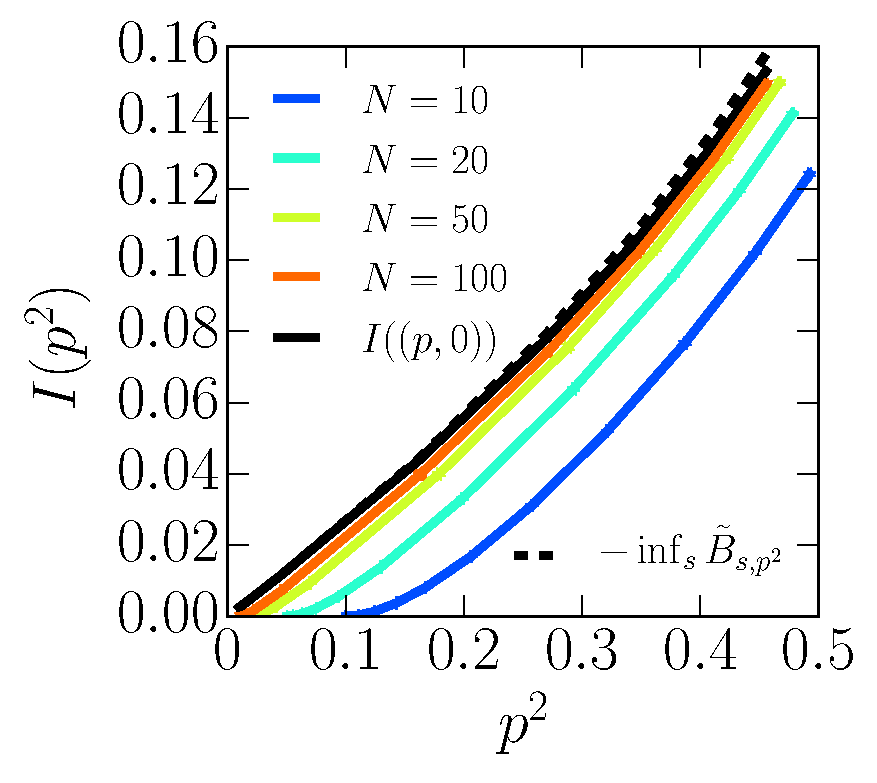
\includegraphics[width=0.40\textwidth]{rate_cloning.eps}
\caption{\textbf{(left)} Rate function. -- Using \textsc{Mathieu} in \href{https://github.com/yketa/active_work/blob/master/rotors.py}{\faGithub~ yketa/active\_work/rotors.py}. \textbf{(right)} Comparison to numerics -- $N_{\mathrm{clones}} = 10^3$, $t_{\mathrm{max}} = 10^2$.}
\label{mathieu_rate_fig}
\end{figure}

\section{Optimal control potential}

We have that the tilted generator is self-adjoint (hermitian), so that the left and right eigenfunctions are identical. We thus have the eigenfunction for the $\bm{s} \parallel \bm{e}_x$ problem,
\begin{equation}
\mathcal{F}_s(\theta) \propto y_{Mathieu, 0}\left(\frac{\theta}{2}, \frac{2s}{D_r}\right)
\end{equation}
with $y_{Mathieu, 0}$ the $0$-th Mathieu function, even and $\pi$-periodic, so that $\mathcal{F}_s(\theta)$ is $2\pi$-periodic, associated to the eigenvalue $\psi_{p}(s)$. We can thus compute the optimal control potential \cite{jack2019ergodicity}
\begin{equation}
\phi_s(\theta) = - 2 \log \mathcal{F}_s(\theta)
\end{equation}
to achieve the fluctuations characteristic to the biased trajectories. We can compute the curvature of this potential at $$\theta = 0$$,
\begin{equation}
\left. \frac{\partial^2}{\partial \theta^2} \phi_s(\theta) \right|_{s=0} = 2 \left(\mathcal{F}(\theta = 0)^{-2} \left(\frac{\partial}{\partial \theta} \mathcal{F}(\theta = 0)\right)^2 - \mathcal{F}(\theta = 0)^{-1}\frac{\partial^2}{\partial\theta^2} \mathcal{F}(\theta = 0)\right),
\end{equation}
where
\begin{equation}
\frac{\partial}{\partial \theta} \mathcal{F}(\theta = 0) = 0,
\end{equation}
by parity of $y_{Mathieu, 0}$, and
\begin{equation}
\begin{aligned}
- \mathcal{F}(\theta = 0)^{-1}\frac{\partial^2}{\partial\theta^2} \mathcal{F}(\theta = 0) &= \left. - y_{Mathieu, 0}\left(\frac{\theta}{2}, \frac{2s}{D_r}\right)^{-1}\frac{\partial^2}{\partial\theta^2} y_{Mathieu, 0}\left(\frac{\theta}{2}, \frac{2s}{D_r}\right) \right|_{\theta=0}\\
&= \frac{1}{4} \left(a_{\mathrm{Mathieu}, 0}\left(\frac{2s}{D_r}\right) - 2 \frac{2s}{D_r}\right)
\end{aligned}
\end{equation}
from the differential equation defining $y_{Mathieu, 0}$ (Eq. (\ref{1P_eigenproblem})), therefore
\begin{equation}
\left. \frac{\partial^2}{\partial \theta^2} \phi_s(\theta) \right|_{s=0} = \frac{1}{2} \left(a_{\mathrm{Mathieu}, 0}\left(\frac{2s}{D_r}\right) - 2 \frac{2s}{D_r}\right),
\end{equation}
so we can compare this optimal potential to a potential $\phi^{(g)}_s \propto g (1 - \cos\theta)$,
\begin{equation}
\phi^{(g)}_s(\theta) = \frac{1}{2} \left(a_{\mathrm{Mathieu}, 0}\left(\frac{2s}{D_r}\right) - 2 \frac{2s}{D_r}\right) (1 - \cos\theta),
\end{equation}
of identical curvature at $\theta = 0$ (see Fig. \ref{mathieu_potential_fig}).

\begin{figure}[H]
\centering
\includegraphics[width=0.40\textwidth]{mathieu_potential.eps}
\caption{Optimal control potential. -- Using \textsc{Mathieu} in \href{https://github.com/yketa/active_work/blob/master/rotors.py}{\faGithub~ yketa/active\_work/rotors.py}.}
\label{mathieu_potential_fig}
\end{figure}

\bibliographystyle{unsrt}
{\renewcommand{\bibname}{References}\bibliography{ref}}

\end{document}
